% !TEX spellcheck = en_US
% !TEX spellcheck = LaTeX
\documentclass[letterpaper,english,10pt]{article}
\usepackage{%
	amsfonts,%
	amsmath,%	
	amssymb,%
	amsthm,%
	babel,%
	bbm,%
	%biblatex,%
	caption,%
	centernot,%
	color,%
	enumerate,%
	%enumitem,%
	epsfig,%
	epstopdf,%
	etex,%
	fancybox,%
	framed,%
	fullpage,%
	%geometry,%
	graphicx,%
	hyperref,%
	latexsym,%
	mathptmx,%
	mathtools,%
	multicol,%
	pgf,%
	pgfplots,%
	pgfplotstable,%
	pgfpages,%
	proof,%
	psfrag,%
	%subfigure,%	
	tikz,%
	times,%
	ulem,%
	url,%
	xcolor,%
	mathpazo
}

\definecolor{shadecolor}{gray}{.95}%{rgb}{1,0,0}
\usepackage[margin=1in,top=0.75in]{geometry}
\usepackage[mathscr]{eucal}
\usepgflibrary{shapes}
\usepgfplotslibrary{fillbetween}
\usetikzlibrary{%
  arrows,%
  backgrounds,%
  chains,%
  decorations.pathmorphing,% /pgf/decoration/random steps | erste Graphik
  decorations.text,% 
  matrix,%
  positioning,% wg. " of "
  fit,%
  patterns,%
  petri,%
  plotmarks,%
  scopes,%
  shadows,%
  shapes.misc,% wg. rounded rectangle
  shapes.arrows,%
  shapes.callouts,%
  shapes%
}

%\pgfplotsset{compat=newest} %<------ Here
\pgfplotsset{compat=1.11} %<------ Or use this one

\theoremstyle{plain}
\newtheorem{thm}{Theorem}[section]
\newtheorem{lem}[thm]{Lemma}
\newtheorem{prop}[thm]{Proposition}
\newtheorem{cor}[thm]{Corollary}
\newtheorem{clm}[thm]{Claim}

\theoremstyle{definition}
\newtheorem{axiom}[thm]{Axiom}
\newtheorem{defn}[thm]{Definition}
\newtheorem{conj}[thm]{Conjecture}
\newtheorem{exmp}[thm]{Example}
\newtheorem{exerc}[thm]{Exercise}
\newtheorem{assum}[thm]{Assumptions}

\theoremstyle{remark}
\newtheorem{rem}[thm]{Remark}
\newtheorem{note}[thm]{Note}

\newcommand{\Cov}{\operatorname{Cov}}
%\newcommand{\det}{\operatorname{det}}
\newcommand{\Real}{\mathbb{R}}
\newcommand{\tr}{\operatorname{tr}}
%\newcommand{\Var}{\operatorname{Var}}

\DeclareMathOperator{\sign}{sign}
%\renewcommand{\proof}[1]{\begin{proof}#1\end{proof}}
\newcommand{\EQ}[1]{\begin{equation*}#1\end{equation*}}
\newcommand{\EQN}[1]{\begin{equation}#1\end{equation}}
\newcommand{\eq}[1]{\begin{align*}#1\end{align*}}
\newcommand{\meq}[2]{\begin{xalignat*}{#1}#2\end{xalignat*}}
\newcommand{\norm}[1]{\left\lVert#1\right\rVert}
\newcommand{\abs}[1]{\left\lvert#1\right\rvert}
\newcommand{\expect}[1]{\mathbb{E}\left[{#1}\right]}
\newcommand{\prob}[1]{\mathbb{P}\left[{#1}\right]}
\newcommand{\given}{\; \big\vert \;} 
\newcommand{\set}[1]{\left\{#1\right\}} 
\newcommand{\indicator}[1]{\mathbb{1}_{\set{#1}}} 
\newcommand{\inner}[1]{\left\langle#1\right\rangle}
\newcommand{\red}[1]{\textcolor{red}{#1}} 
\newcommand{\E}[1]{\mathbb{E}\left[#1\right]}
\newcommand{\Var}[1]{\operatorname{Var}\left[#1\right]}

\newcommand{\D}{\mathbb{D}}
%\newcommand{\E}{\mathbb{E}}
\newcommand{\N}{\mathbb{N}}
\renewcommand{\P}{\mathbb{P}}
\newcommand{\Q}{\mathbb{Q}}
\newcommand{\R}{\mathbb{R}}
\newcommand{\Z}{\mathbb{Z}}

\newcommand{\bU}{\mathbf{1}}
\newcommand{\bx}{\mathbf{x}}

\newcommand{\cB}{\mathcal{B}}
\newcommand{\cC}{\mathcal{C}}
\newcommand{\cD}{\mathcal{D}}
\newcommand{\cF}{\mathcal{F}}
\newcommand{\cG}{\mathcal{G}}
\newcommand{\cH}{\mathcal{H}}
\newcommand{\cO}{\mathcal{O}}
\newcommand{\cT}{\mathcal{T}}
\newcommand{\cX}{\mathcal{X}}
\newcommand{\cY}{\mathcal{Y}}

\newcommand{\sA}{\mathscr{A}}
\newcommand{\sB}{\mathscr{B}}
\newcommand{\sC}{\mathscr{C}}
\newcommand{\sD}{\mathscr{D}}
\newcommand{\sE}{\mathscr{E}}
\newcommand{\sF}{\mathscr{F}}
\newcommand{\sG}{\mathscr{G}}
\newcommand{\sH}{\mathscr{H}}
\newcommand{\sL}{\mathscr{L}}
\newcommand{\dO}{\mathscr{O}}
\newcommand{\sS}{\mathscr{S}}
\newcommand{\sT}{\mathscr{T}}
\newcommand{\sX}{\mathscr{X}}
\newcommand{\sY}{\mathscr{Y}}
\newcommand{\sZ}{\mathscr{Z}}

% Debug
\newcommand{\todo}[1]{\begin{color}{blue}{{\bf~[TODO:~#1]}}\end{color}}

% a few handy macros

\renewcommand{\le}{\leqslant}
\renewcommand{\ge}{\geqslant}
\newcommand\matlab{{\sc matlab}}
\newcommand{\goto}{\rightarrow}
\newcommand{\bigo}{{\mathcal O}}
%\newcommand{\half}{\frac{1}{2}}
%\newcommand\implies{\quad\Longrightarrow\quad}
\newcommand\reals{{{\rm l} \kern -.15em {\rm R} }}
\newcommand\complex{{\raisebox{.043ex}{\rule{0.07em}{1.56ex}} \hskip -.35em {\rm C}}}


% macros for matrices/vectors:

% matrix environment for vectors or matrices where elements are centered
\newenvironment{mat}{\left[\begin{array}{ccccccccccccccc}}{\end{array}\right]}
\newcommand\bcm{\begin{mat}}
\newcommand\ecm{\end{mat}}

% matrix environment for vectors or matrices where elements are right justifvied
\newenvironment{rmat}{\left[\begin{array}{rrrrrrrrrrrrr}}{\end{array}\right]}
\newcommand\brm{\begin{rmat}}
\newcommand\erm{\end{rmat}}

% for left brace and a set of choices
%\newenvironment{choices}{\left\{ \begin{array}{ll}}{\end{array}\right.}
\newcommand\when{&\text{if~}}
\newcommand\otherwise{&\text{otherwise}}
% sample usage:
%  \delta_{ij} = \begin{choices} 1 \when i=j, \\ 0 \otherwise \end{choices}


% for labeling and referencing equations:
\newcommand{\eql}{\begin{equation}\label}
\newcommand{\eqn}[1]{(\ref{#1})}
% can then do
%  \eql{eqnlabel}
%  ...
%  \end{equation}
% and refer to it as equation \eqn{eqnlabel}.  


% some useful macros for finite difference methods:
\newcommand\unp{U^{n+1}}
\newcommand\unm{U^{n-1}}

% for chemical reactions:
\newcommand{\react}[1]{\stackrel{K_{#1}}{\rightarrow}}
\newcommand{\reactb}[2]{\stackrel{K_{#1}}{~\stackrel{\rightleftharpoons}
   {\scriptstyle K_{#2}}}~}


\makeatletter
\def\th@plain{%
  \thm@notefont{}% same as heading font
  \itshape % body font
}
\def\th@definition{%
  \thm@notefont{}% same as heading font
  \normalfont % body font
}
\makeatother
\date{}


\title{Lecture-20: The Random Code Ensemble}


\begin{document}
\maketitle

\section{Geometry}

The relevant geometry for binary error-correcting codes is that of \textbf{Hamming space}. 
The $N$-dimensional binary Hamming space is the metric space defined by the set  $\set{0,1}^N$ and the Hamming metric
\EQ{
d(x,z) \triangleq \sum_{i=1}^N\indicator{x_i \neq z_i}.
}
Let us define the distance enumerator of a code $\fC$, relative to the codeword $z$, to be
\EQ{
\cN_z(h) \triangleq \abs{\set{x \in \fC: d(x,z) = h}},~ h \in [N].
}
For $ z = x^{(m)}$, this quantity is closely related to the conditional probability of decoding error given that $x^{(m)}$ is sent.
For the RCE, the quantity $\cN_{X^{(0)}}(h)$ is a random variable and we can easily determine its expected value. 
In particular, we have 
\eq{
\E \cN_{X^{(0)}}(h) &= \E\sum_{m \in \set{0,1}^M}\indicator{d(X^{(0)}, X^{(m)}) = h} = \indicator{h=0} + \sum_{m \in \set{0,1}^M\setminus 0}P\set{d(X^{(0)}, X^{(m)}) = h}\\
&= \indicator{h=0} + \sum_{m \in \set{0,1}^M\setminus 0}2^{-N}\binom{N}{h} 
=  \indicator{h=0} + (2^M-1)2^{-N}\binom{N}{h} \le 2^{M-N}\binom{N}{h}
}
for $h  \ge 1$. 
For a non-negative integer random variable $Z$, one has $P\set{Z \ge 1} \le \E Z$ (Markov's inequality). 
This implies that
\EQ{
P\set{\cN_{X^{0}}(h) \ge 1} \le 2^{M-N}\binom{N}{h},~~h \ge 1.
}
Since $d(X^{(0)},X^{(m)})$ is invariant under translation, 
the uniform distribution of $X^{(m)}$ for $m \neq 0$ implies that this result is completely independent of $X^{(0)}$
To analyze the asymptotics, we choose $M=\lfloor RN\rfloor$ with $R \in (0,1)$ and $h = \lfloor\delta N\rfloor$ with
$\delta \in (0,1)$. 
The quantity $\delta$ is called the \textbf{normalized} distance or weight of the codeword. 
In this case, 
\EQ{
\binom{N}{\lfloor{\delta N\rfloor}} \stackrel{\cdot}{=} 2^{N\cH(\delta)}. 
}
implies that 
\EQ{
P\set{\cN_{X^{(0)}}(\lfloor \delta N\rfloor) \ge 1} \le \E\cN_{X^{(0)}}(\lfloor \delta N\rfloor) \stackrel{\cdot}{=} 2^{N(R-1+\cH(\delta))}. 
}
If $R-1+\cH(\delta) < 0$, then the probability that a random codeword has another codeword closer than distance $\delta N$ is decreasing exponentially fast to $0$. 
Thus, the typical minimum distance, which is called the \textbf{Gilbert-Varshamov distance} and denoted by $\delta_{GV}(R)$ is given by the smallest root of $R-1+\cH(\delta)$. 
For example, $\delta_{GV}(1/2) = 0.11$. 

The quantity $r_N(\delta) = \frac{1}{N}\log_2\cN_{X^{(0)}}(\lfloor\delta N\rfloor)$ is also important in the analysis of code ensembles. 
It is often called the \textbf{exponential growth rate} or \textbf{spectral shape} of the ensemble. 
For the RCE, one can also show that $r_N(\delta)$ is concentrated around its asymptotic expectation $r(\delta) \triangleq ?? R-1+\cH(\delta)$ for all $\delta$ such that $r(\delta) > 0$. 
In particular, for any $\epsilon > 0$ and all $\delta \in (\delta_{GV}(R), 1 - \delta_{GV}(R))$, we have
\EQ{
\lim_{N\to\infty}P\set{\abs{\frac{1}{N}\log_2\cN_{X^{(0)}}(\lfloor \delta N\rfloor) - r(\delta)}>\epsilon} = 0.
}
\section{The binary symmetric channel}
\begin{figure}[h!]
    \centering
    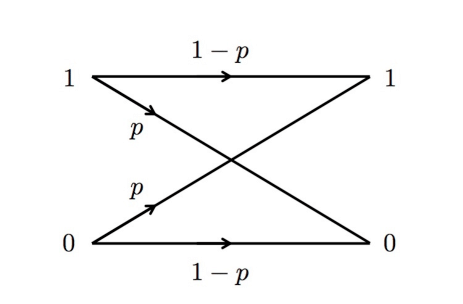
\includegraphics[scale=0.4]{Figures/bscp.png}
    \caption{Representation of BSC(p)}
    \label{fig:my_label}
\end{figure}
\flushleft The binary symmetric channel (BSC) with error probability $p$ is denoted by BSC($p$). 
This channel flips an input bit with probability $p$ and leaves it unchanged with probability $1 - p$. 
This implies that 
\EQ{
Q(y|x) = \begin{cases}
1-p, & x = y,\\
p, & x \neq y.
\end{cases}
}
\subsection{Word-MAP decoding}
For the BSC($p$) channel, we can rewrite the posterior probability distribution of input $x$ given observation $y$ as 
\EQ{
\mu_y(x)= \frac{1}{Z(y)}p^{d(x,y)}(1-p)^{N-d(x,y)}\frac{1}{\abs{\fC}}\indicator{x \in \fC} \propto \left(\frac{p}{1-p}\right)^{d(x,y)}\indicator{x \in \fC}.
}
Thus, if $p < 1/2$, the MAP codeword is precisely the codeword $x$ that minimizes the Hamming distance $d(x, y)$ (i.e., the closest codeword to the received sequence). 
Based on the geometry of the RCE, we know that w.h.p. the transmitted codeword is the unique codeword in a ball of radius $\delta_{GV}(R)N$ around the transmitted codeword. 
This also implies that, if we consider balls of radius $\delta_{GV}(R)N/2$ around each codeword, then only a vanishing fraction of these balls intersect each other. 
Thus, one can expurgate (i.e., delete) a vanishing fraction of codewords to make all of these balls are disjoint.\begin{figure}[h!]
    \centering
    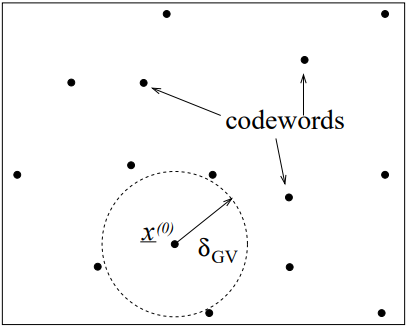
\includegraphics[scale=0.5]{Figures/RCE2.png}
    \caption{No codewords in $\delta_{GV}$ distance but exponentially many outside the hamming ball of radius $\delta_{GV}$ }
    \label{fig:my_label}
\end{figure}  
This expurgated code will correct all error patterns with fewer than $\delta_{GV}(R)N/2$ errors.
It turns out that one can actually handle twice as many errors. 
To see this, we observe two things. 
First, the Hamming distance from the transmitted codeword to the received codeword $d(X^{(0)},Y)$ is a sum of i.i.d. Bernoulli-$p$ random variables and it satisfies the law of large numbers, 
\EQ{
\lim_{N\to\infty}P\set{\abs{\frac{1}{N}d(X^{(0)},Y) -p}>\epsilon}= 0.
}
Second, for any $\delta < \delta_{GV}(R)$, it holds that 
\EQ{
\lim_{N\to\infty}P\set{\frac{1}{N}\min_{m \in \set{0,1}^M\setminus 0}d(X^{(m)},Y)<\delta}= 0.
}
Since the analysis in the previous Section is independent of the distribution of $X^{(0)}$, 
this follows directly from analyzing the minimum distance of a code where $X^{(0)}$ is replaced by $Y$. 
Putting these together, we see that $p < \delta_{GV}(R)$ is sufficient w.h.p. for the correct codeword to be the closest codeword to the received vector. 
Applying $1 - \cH(\cdot)$ to both sides, 
this can be rewritten as $R < C_{BSC}(p) = 1- \cH(p)$ where $C_{BSC}(p)$ is the capacity of the BSC($p$). 
Thus, we have verified that the RCE achieves capacity on the BSC under Word-MAP decoding.
\begin{figure}
    \centering
    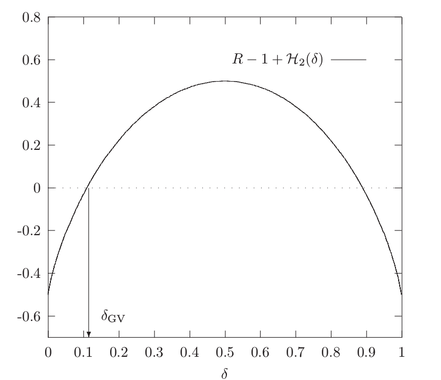
\includegraphics[scale=0.6]{Figures/RCE.png}
    \caption{Growth rate of the distance enumerator for the random code ensemble
with rate R = 1/2 as a function of the Hamming distance $d = N\delta$.}
    \label{fig:my_label}
\end{figure}

\section{Connections with statistical physics}
\subsection{The Random Energy Model}
The random energy model (REM) assumes the binary vectors ${0,1}^M$ are randomly associated with $2^M$ i.i.d. random variables drawn from a well-behaved distribution whose variance grows linearly with M (e.g., a Gaussian distribution with variance M/2).
For the BSC(p) channel with transmitted codeword $x = X^{(0)}$ and received vector y, the Hamming distances to incorrect codewords, 
\EQ{E_m= d(y,X^{(m)})\quad \text{for m} \neq 0,}
 are independent random variables with the binomial distribution
\EQ{P(E_m =k)= {\frac{1}{2}}^N \binom{N}{k}}
Thus, the distance between the received vector and the closest incorrect codeword is given by
\EQ{\min_{m'\in \set{0,1}^M}E_m' }     
This quantity is exactly the ground state energy of the  Random Energy Model with the binomial energy dis- tribution. When normalized by 1/N, this energy concentrates around the value $\delta_{GV}(R)$. Similarly, the distance between the received vector and the correct codeword, when normalized by 1/N, concentrates around the value p. Thus, \textbf{decoding will be successful if and only if} 
\EQ{p < \delta_{GV}(R)}.
\subsection{The Boltzmann Distribution}
Suppose we think about the decoding problem as a spin system where the energy of configuration x is given by
\EQ{
E(x) = \begin{cases}
-ln(Q(y/x)), & x \in \fC,\\
\infty, & otherwise.
\end{cases}
}
In this case, the Boltzmann distribution for inverse temperature is given by
\EQ{\mu_{\beta}(x)=\frac{1}{z(\beta)}e^{-\beta E(x)}=\frac{{Q(y/x)}^\beta}{z(\beta)}
}

\end{document}


\subsection{An Intuitive approach for general channels}
Another interpretation of the above analysis is that each output sequence within normalized distance $\delta < \delta_{GV}(R)$ of a codeword has w.h.p. no other codewords within normalized distance $\delta$. 
This means that we can design a decoder using the following rule. 
Each received sequence is associated with an arbitrary codeword within normalized distance $\delta$, 
if such a codeword exists. 
The resulting decoder simply maps the received sequence to its associated codeword. 
For any $\epsilon > 0$ and transmission over the BSC($p$) channel with $p = \delta-\epsilon$, this decoder will succeed w.h.p. as $N \to \infty$. 
For general channels, one can use roughly the same idea. 
The main difference is the size of relevant objects is measured using entropies. 
The key ingredient is that, for i.i.d. sequences $(X_1,  \dots, X_N )$ with large $N$, the probability distribution essentially becomes uniform over a set of 2NH(X) ?typical? sequences. Similarly, for (X,Y) ? p(x)Q(y|x), the i.i.d. sequence ((X1,Y1),...,(XN,YN))takesoneof2NH(X,Y) differenttypicalvalueswithessentiallyuni- form probability and the number of (Y1, . . . , YN ) typical sequences is roughly 2NH(Y ). Also, if we fix the (X1,...,XN) sequence to a typical value (x1,...,xN), then the number of ((x1,Y1),...,(xN,YN))typicalsequencesisroughly2NH(Y|X). Thislastsetofsequencescan be seen as the likely set of output sequences when x is transmitted.
    
To use these ideas, we start by drawing 2NR codewords X(m) whose entries are i.i.d. distributed according to p(x). For each of these codewords, we enumerate the 2NH(Y|X) typical output sequences and associate each one with the transmitted codeword. Some received values may associated with multiple codewords but the following calculation shows this is not likely. For any output sequence y that is associated with at least one codeword, we can upper bound the total number of codewords with which it is associated. Let Am be the indicator random variable for the event that X(m) is associated with y. For simplicity, assume that y is in the typical output set associated with codeword X(0). The key is to observethattherandomvariablesA1,A2,...,A2M?1 arei.i.d.with
\end{document}

9
      P (Am = 1) =. 2N[H(Y |X)?H(Y )] = 2?NI(X;Y ). ????
This implies that
???? P ?? Am ?1 ?E ?? Am
= ?? P(Am =1)=. 2N[R?I(X;Y)]. m?{0,1}M \0
m?{0,1}M \0
m?{0,1}M \0
   Thus, if R < I (X; Y ) and the codeword x is transmitted then w.h.p. a randomly chosen typical output sequence y will be associated with the transmitted codeword x. By symmetry, the same statement holds for all codewords and decoding succeeds with high probability.
C. Bit-MAP Decoding
For Bit-MAP decoding, the i-th bit is decoded by first computing its posterior marginal and then maximizing. First, we note that the Bit-MAP decoder is equal to the Word-MAP decoder if there is an x? ? C such that ?y(x?) > 1/2. This is because the contribution of ?y(x?) to
?(i)(x ) = ??? (x) yiy
x\i
is enough to guarantee that ?(i)(x?) > 1/2. To analyze this, we consider the posterior
        probability
yi
exp ???d(x, y) ln 1?p ??
  ?y(x) = ?? ??x??C exp
p ?d(x?, y) ln p
1?p??.
       
Since the spectral shape of the RCE is concentrated around its expectation whenever it is positive, it follows that
????? 1?p?? Z= exp ?d(x,y)ln p
?? 1 ? p?? N?N?GV(R) h=N ?GV (R)
?? ??
exp N R?1+He ??
?? h ?????? N
??
exp ?hln
1 ? p?? p
.
. ?? 1?p?? ??
R?1+He(?)??ln ifp<?GV(R)
1?p???? p
10
   x? ?C
=exp ?Npln p + ??
    =exp ?Npln +exp N p
max
p
  ?GV (R)???1??GV (R) ???1?p???? 1?p??
=. ??exp ?Npln p +exp ?N?GV(R)ln p ??exp???Npln1?p??+exp(?N(R?1?ln(1?p))) ifp?[?GV(R),1/2].
   In the first case, the maximum is achieved by ?? = ?GV(R) due to the boundary constraint and, in the second case, one finds that ?? = p. For p < ?GV(R), we can plug this into the original formula to see that ?y(x) ? 1 w.h.p. when x is the transmitted codeword. This implies that the Bit-MAP decoder will also give the right answer w.h.p. if p < ?GV(R).
For p > ?GV(R), the previous calculation also shows that Z is determined by the roughly
exp(N[R ? 1 + He(p)]) dominant codewords at distance roughly Np from y. To analyze the
Bit-MAP decoder, we can use the following trick. If we make the code one bit longer, then
the new codeword bits (i.e., bit N + 1) in each codeword are i.i.d. random variables that
are independent of the previous code bits and the N received values we have already seen.
Thus, for all codewords except the transmitted codeword, the probability that the new code
bit xN+1 equals the received value yN+1 is 1. Let n= (resp. ?=) be the number of dominant 2
codewords with xN+1 = yN+1 (resp. xN+1?= yN+1). This implies that the ratio n=/?= will concentrate sharply around 1 whenever these numbers are growing with N.
Let Z= (resp. ?=) be the partition function for the Word-MAP decoder of the length-
N + 1 code summed over all codewords where xN+1 = yN+1 (resp. xN+1?= yN+1). Based on
the above arguments, it follows that Z= =. Zn= and ?= =. Z?= p , where Z is the partition 1?p
function of the Word-MAP decoder for the length-N code. Thus, we can write ?(N+1)(y ) = Z= =. Zn= ? 1 ? p.
     y N+1 Z=+?= Zn=+Z?= p 1?p
   This is exactly the same answer as one would get decoding xN+1 from the single observation yN+1. The reason is that the dominant codewords for the length-N Word-MAP decoder

11 essentially have a random value of bit N + 1 and the first N received bits provide essentially
no information about xN+1.
VI. CONNECTIONS WITH STATISTICAL PHYSICS
A. The Random Energy Model
The random energy model (REM) assumes the binary vectors, {0,1}M, are randomly associated with 2M i.i.d. random variables drawn from a well-behaved distribution whose variance grows linearly with M (e.g., a Gaussian distribution with variance M/2). For the BSC(p) channel with transmitted codeword x = X(0) and received vector y, the Hamming distances to incorrect codewords, Em = d??y,X(m)?? for m?= 0, are independent random variables with the binomial distribution
??N??
      P(Em =k)=2?N
Thus, the distance between the received vector and the closest incorrect codeword is given
by
minM Em. m? ?{0,1} \0
This quantity is exactly the ground state energy of the REM with the binomial energy dis- tribution. When normalized by 1/N, this energy concentrates around the value ?GV(R). Similarly, the distance between the received vector and the correct codeword, when normal- ized by 1/N, concentrates around the value p. Thus, decoding will be successful if and only if p < ?GV(R).
B. The Boltzmann Distribution
Suppose we think about the decoding problem as a spin system where the energy of configuration x is given by
?
???lnQ(y|x) if x ? C
E(x) =
??? otherwise.
In this case, the Boltzmann distribution for inverse temperature ? is given by
1 ??E(x) Q(y|x)? ??(x) = Z(?)e = Z(?) ,
k
.
            
         2.5 2 1.5 1 0.5 0
paramagnetic
Communicating over a binary symmetric channel
12
       1/?
ordered
0.1 0.2
glassy
      where
Figà 6à5 Phase diagram for the rate- 2 random code ensemble over a binary symmetric channel, using Þnite temperature decodingà Word MAP and bit MAP decoding correspond to  ? = à and  ? = , respectivelyà Note that the phase boundary of the error-free ordered phase is vertical in this interval of temperatureà
to 1 as N ? ?. The measure ?y,?(x) is dominated by the codewords closest to the received message y (which are distinct from the correct codeword, since p > ?GV(R)). Its Shannon entropy H(?y,?) is sublinear in N. This situation is closely related to the ?measure condensation? phenomenon that occurs in the low-temperature phase of the random energy model.
0
0.3 0.4 0.5
p
Z(?) = ?? e??E(x). (3) 3. An ?entropy-dominated? (paramagnetic) phase at high temperature (small enough
 ?). The bit and block error rates behave as in the glassy phase, and ?y,?(x à ) = x?{0,1}N
exp{??(N)}. However, the measure ?y,?(x) is now dominated by codewords whose distance d ? N?? from the received message is larger than the minimal
 If ? = 1, then ??(x) is edixstancet:l?y
? = 0. In the first case we recover the result already obtained for symbol MAP
?=thpe/[po+s(1te?rpi)o]r.Indpiasrtircuiblaru,t??
???
?
n=s1m/2ifttedcodewordgiven
words, and the distance from the received message under this distribution is, with
high probability, close to N/2. In this regime, the Shannon entropy H(??) is linear support.If?>1,theinNt.hedistributionistiltedtowardsauniformdistributionoverits
Finite-temperature decoding can be generalized to other channel models. Let ?y(x)
maximizers. Thus,abseth?ed?istribu?tion,otfhthetrWansmoirttded-MmesAsagPecodndeitciondaleonrthieschwanenelllo-uatpupt,rgiovexnimatedbyasample
explicitly in eqn (6.5). For ? > 0, we define the distribution form the Boltzmann distribution.
1The partition function Z(?) defined here differs by a multiplicative constant from the one defined in eqn (6.26) for a BSC.
As we saw earlier, w.h.p. this sample will be the correct answer only if p < ?
p > ?GV(R), there is an additional change in behavior that can occur as one changes ?. In particular, one can ask whether or not the set of dominant codewords in (3) grows exponen- tially. If it grows exponentially, then the system is in a high temperature (or ?paramagnetic?) phase. If it does not grow exponentially, then the measure has condensed onto a set with sublinear entropy and the system is in a ?glassy? phase. To get a qualitative understanding of this distinction, look at the above figure and then ask Patrick more about spin glasses in class.
\end{document}
